\documentclass[oldversion]{aa}
%\documentclass[referee]{aa}
\usepackage{epsfig}
\usepackage{natbib}
\usepackage{lscape}
\usepackage{wasysym}
\usepackage{amssymb}
\usepackage{subfigure}
%\usepackage{multicol}
\usepackage{longtable}
\usepackage{rotating}
\usepackage{color}
\usepackage{colortbl}
\usepackage{fancyheadings}
\bibpunct{(}{)}{;}{a}{}{,}

\newcommand\T{\rule{0pt}{2.6ex}}
\newcommand\B{\rule[-1.2ex]{0pt}{0pt}}

\begin{document}

\title{A comparative test of metallicity calibrations for M dwarfs \thanks{Based on observations collected with the FEROS, ELODIE and SOPHIE spectrographs under the programs 060.A-9120(B), 073.D-0802(A), 074.D-0670(A)}}
%\subtitle{}



\author{ V. Neves\inst{1,2} \and X. Bonfils\inst{2} \and N. C. Santos\inst{1,3} \and X. Delfosse\inst{2} \and T. Forveille\inst{2}  \and F. Allard\inst{4}  \and C. Nat\'ario\inst{5,6} \and C. S. Fernandes\inst{5} \and S. Udry\inst{7}}

\institute{
Centro de Astrof{\'\i}sica, Universidade do Porto, Rua das Estrelas, 4150-762 Porto, Portugal \\
email: {\tt vasco.neves@astro.ua.pt}
\and
UJF-Grenoble 1 / CNRS-INSU, Institut de Plan\' etologie et d�Astrophysique de Grenoble (IPAG) UMR 5274, Grenoble, F-38041, France.
\and
Departamento de F{\'i}sica e Astronomia, Faculdade de Ci{\^e}ncias, Universidade do Porto, Portugal
\and
Centre de Recherche Astrophysique de Lyon, UMR 5574: CNRS, Universit\'e de Lyon, \'Ecole Normale Sup\'erieure de Lyon, 46 All\'ee d'Italie, F-69364 Lyon Cedex 07, France
\and
Centro de Astronomia e Astrof\'isica da Universidade de Lisboa, Campo Grande, Ed. C8 1749-016 Lisboa, Portugal
\and
Leiden Observatory, Leiden University, The Netherlands
\and
Observatoire de Gen\`eve, Universit\'e de Gen\`eve, 51 Chemin des Maillettes, 1290 Sauverny, Switzerland
}


%    Physikalisches Institut, University of Bern, Sidlerstrasse 5, 3012 Bern, Switzerland
%    \and


\date{Received XXX; accepted XXX}

\abstract{We present a comparative test of {\color{red} five metallicity calibrations of M dwarfs proposed in the literature. Our test sample is made of 22 M dwarfs, companion of widely separated ($>$ 5 arcsec) F-, G- or K- dwarfs with known or newly measured metallicity. We included M dwarfs with reliable V photometry only by restricting our sample to stars with V uncertainty lower than $\sim$0.02 dex. Among all calibrations, we find that Schlaufman \& Laughlin (2010) provides lower offset and residuals against our sample and, ultimately, we used that larger sample to update and marginally improve their calibration. Despite better V photometry than used in previous studies the dispersion remains largely in excess given [Fe/H] and photometric uncertainties, suggesting it has physical roots.}

%photometry ($<\pm$xx dex) from the works of Bonfils et al. (2005), Casagrande et al. (2008), Johnson \& Apps (2009), and Schlaufman \& Laughlin (2010), using  a sample of 22 M dwarf companions with {\color{red} a widely separated ($>$ 5 arcsec)} FGK primary. The aim here is to clarify which metallicity calibration should be used when a [Fe/H] estimation of M dwarfs is needed. We conclude that, at present, the best metallicity calibration is the one of Schlaufman \& Laughlin (2010): it has the lowest offset, rms, and explains the variance of the data better. We also find out that the use of precise V photometry does not change the final dispersion of the calibrations of Bonfils et al. (2005), Johnson \& Apps (2009), and Schlaufman \& Laughlin (2010). %In the near future, we intend %to test the Rojas-Ayala et al. calibration, to study  the planet-metallicity correlation, and to create a precise ($\sim$ 0.05 dex) metallicity calibration.

\keywords{stars: abundances -- 
stars: fundamental parameters -- 
stars: planetary systems -- 
stars: late type
stars: atmospheres
}
	    }

\authorrunning{Neves et al.}
\titlerunning{A comparative test of metallicity calibrations for M dwarfs}
\maketitle

\section{Introduction}

%M dwarfs are the smallest and coldest stars of the main sequence. However, they are the most numerous and comprise most of its baryonic matter in the Galaxy. (\textcolor{red}{verificar referencia de Chabrier}). 
{\color{red}
In recent times increased interest in M dwarfs has come from planet search programs. Putative planets induce larger reflex velocities and transit depths when they orbit and transit M dwarfs, compared to FGK stars. Lower mass, smaller and possibly habitable planets are therefore easier to find around them, and are indeed detected at an increasing pace \cite[e.g.][]{Udry-2007b, Mayor-2009, Charbonneau-2009}.
 
%of given massLower mass planets around them. In fact, the lower mass and radius of M dwarfs imply that the reflex velocities induced by planets around them, as well as the transit depths, are considerably larger, when compared to the same effects induced in the more massive, and better studied, FGK stars. Moreover, the habitable zone around these stars is situated in tighter orbits, which makes the detection of planets in this area easier with radial velocity and transit techniques, as both have their best sensitivity closer to the host star (e.g. \citeauthor{Udry-2007b} \citeyear{Udry-2007b}; \citeauthor{Nutzman-2008} \citeyear{Nutzman-2008};  \citeauthor{Mayor-2009} \citeyear{Mayor-2009}).

%M stars are also increasingly important in the context of planet formation around very low mass stars. Some theoretical models predict that the formation of giant planets is seriously inhibited around the less massive stars (M$_{*} <$ 0.4M$_{\odot}$) (e.g. \citeauthor{Laughlin-2004} \citeyear{Laughlin-2004}; \citeauthor{Ida-2005} \citeyear{Ida-2005}). According to them, the formed rocky or ice cores do not have enough time to get a gas envelope and become super-earths or ice giants instead. Others suggest that the proto-planets may have enough time to grow and to accrete the gas envelope before the disk vanishes, by invoking migration and faster accretion (e.g. \citeauthor{Alibert-2005} \citeyear{Alibert-2005}). Alternatively, \citet{Boss-2006a}, and \citet{Boss-2006b} show that the disk instability hypothesis can also play a role in the formation of planets around M dwarfs. Indeed, an increasingly number of planets are being detected around these stars and they show that most planets have, on average, a lower mass than those found on FGK stars, the majority being Neptunians and super-Earths (e.g. \citeauthor{Bonfils-2007} \citeyear{Bonfils-2007}; \citeauthor{Udry-2007b} \citeyear{Udry-2007b} \textcolor{red}{mais 1 ou 2 referencias aqui}). 

%On the observational side, M dwarfs are under considerable attention as planet hosts: 

From the ever growing number of exoplanets emerges interesting statistical properties of their characteristics or the characteristics of their host stars (for a review see \citeauthor{Udry-2007} \citeyear{Udry-2007}). Among those, the planet-metallicity correlation is one of the most remarkable : stars with higher metal content have, on average, a higher probability to host Jovian planets (\citeauthor{Gonzalez-1997} \citeyear{Gonzalez-1997}; \citeauthor{Santos-2001a} \citeyear{Santos-2001a}; \citeauthor{Santos-2004b} \citeyear{Santos-2004b}; \citeauthor{Fischer-2005} \citeyear{Fischer-2005}). Within the core-accretion paradigm of the planetary formation, that property is expected to extend to the cooler M dwarfs : to counterbalance the lower mass of their protoplanetary disks, and provide enough material to form planet of similar mass, their density has to increase. And, while the planet-metallicity correlation seems to vanish for FGK stars that host Neptunes and lower-mass planets (\citeauthor{Sousa-2008} \citeyear{Sousa-2008}; \citeauthor{Bouchy-2009} \citeyear{Bouchy-2009}), it might remain persistent for M dwarfs that host Neptune-mass planet.

Probing the planet-metallicity correlation for M dwarfs has largely motivated the first calibration \citep{Bonfils-2005}, but only two M-dwarf hosts were known at the time. More planet detections next allowed to compare the metallicity distributions of M dwarfs {\it with} and {\it without} known planets, and to find they have a $\sim11\%$ probability of being drawn from the same parent distribution \citet{Bonfils-2007}. Today, after even more planets have been detected, and the calibration improved, the probability that M-dwarf hosts are more metal rich than the common M dwarf is evaluated to $\sim6\%$ \citep{Schlaufman-2010}. Although it lines with the core accretion paradigm, the confidence level of that difference remains below 3 $\sigma$. Multiplying the number of known planets and improving metallicity determinations further are therefore the two avenues that must be pursued to better measure the correlation between the stellar metallicity and the planet occurrence for M dwarfs.}


 
%Whether or not this correlation extends to the cooler M dwarfs is still controversial (e.g. \citeauthor{Bonfils-2005} \citeyear{Bonfils-2005}; \citeauthor{Johnson-2009} \citeyear{Johnson-2009}; \citeauthor{Schlaufman-2010} \citeyear{Schlaufman-2010}) and requires very precise measurements. Interestingly, this correlation is likely not observed for FGK stars orbited by Neptune or Super-Earth type planets (\citeauthor{Sousa-2008} \citeyear{Sousa-2008}; \citeauthor{Bouchy-2009} \citeyear{Bouchy-2009}).

%The growing number of exoplanets, as well as a copious amount of high signal-to-noise, high-resolution spectra from their host stars, available from radial velocity surveys, allow the statistical analysis of their properties as well as the properties of their host stars (for a review see \citeauthor{Udry-2007} \citeyear{Udry-2007}). One of the most remarkable correlations found so far for FGK stars that is improving the understanding of the processes of planetary formation is related to the host star: the stars with higher metallicity content have, on average, a higher probability of hosting Jovian class planets (\citeauthor{Gonzalez-1997} \citeyear{Gonzalez-1997}; \citeauthor{Santos-2001a} \citeyear{Santos-2001a}; \citeauthor{Santos-2004b} \citeyear{Santos-2004b}; \citeauthor{Fischer-2005} \citeyear{Fischer-2005}). Whether or not this correlation extends to the cooler M dwarfs is still controversial (e.g. \citeauthor{Bonfils-2005} \citeyear{Bonfils-2005}; \citeauthor{Johnson-2009} \citeyear{Johnson-2009}; \citeauthor{Schlaufman-2010} \citeyear{Schlaufman-2010}) and requires very precise measurements. Interestingly, this correlation is likely not observed for FGK stars orbited by Neptune or Super-Earth type planets (\citeauthor{Sousa-2008} \citeyear{Sousa-2008}; \citeauthor{Bouchy-2009} \citeyear{Bouchy-2009}).


In this paper, we test the photometric metallicity calibrations of \citet{Bonfils-2005}, \citet{Casagrande-2008}, \citet{Johnson-2009}, and \citet{Schlaufman-2010} using  a sample of 22 M dwarf companions with a wide ($>$ 0.5 arcsec) FGK primary. The latest metallicity measurements and calibrations are described in section \ref{latest}. Then, we detail our sample and observations in section \ref{sample}. On section \ref{test}, we test and compare the different calibrations with our measurements. Finally, on section \ref{discussion}, we discuss our results.

\section{The latest metallicity measurements and calibrations}
\label{latest}


For M dwarfs, the measurement of the stellar parameters from their spectra is not a trivial task. As the stellar subtype increases, the number of diatomic and triatomic molecules (e.g. TiO, VO, H$_{2}$O, CO, etc) {\color{red} in their atmospheres increases}, effectively depressing the continuum and making a line-by-line spectroscopic analysis impossible for all but the earlier subtypes. {\color{red} These complex features are not fully reproduce by atmospheric models, themselves limited by incomplete opacity database. In this context, several techniques, more or less successful, have been employed to measure the metal content of M dwarfs.}

{\color{red} \citet{Woolf-2005} measured equivalent widths of atomic lines from high resolution spectra of 35 M and K dwarfs, as classically done for FGK dwarfs, but with updated atmospheric models. Faced by models' limitations, they apply this approach on the M dwarfs with the earliest ($T_{eff} > 3500$ K) and most metal-poor ([Fe/H]$<${\bf XX} dex) subtypes. This study was extended to 32 additional stars \citep{Woolf-2006}, which they used to create a metallicity calibration based on molecular indices, namely CaH2 and TiO5, that can be taken from medium resolution spectra ($\Delta \lambda/\lambda \sim 3000$). {\it This calibration has an uncertainty of $\pm$0.30 dex.} {\bf I don't like that last statement : the goal of the paper is to test the calibrations; we should distinguish better the precision reported by the authors from the precision evaluated by our paper.} {\bf Beside, is it possible to test this calibration with our sample ?}

If the molecular bands render model-based techniques difficult, they have photometric effects that are nevertheless useful to retrieve the metallicity. Increased abundances in TiO and VO shift a large amount of flux from the visible (dominated by the opacities of these species) to the infrared (where the flux is re-radiated). For a given mass, the bolometric luminosity is concurrently diminished when the metallicity increases. Both effects work together in the visible and largely cancel in the infrared, such that the V magnitude is largely dependent on metallicity while infrared magnitudes are not \citep{Chabrier-2000, Delfosse-2000}. \citet{Bonfils-2005} et al. used that effect as a metallicity scale, and to calibrate that scale, they used binary (or multiple) stars with a FGK primary and an M dwarf secondary. The metallicity was measured on the primaries with a classical line-by-line analysis and assumed to be the same for the M-dwarf components. }


%\textbf{An alternative approach, introduced by \citet{Bonfils-2005}, is based on the measurement of metallicities from FGK high-resolution spectra in binary or multiple systems where one of the lesser bright stars is an M dwarf. The metallicity of the latter is inferred from the former. Then, a photometric metallicity calibration is established, based on the fact that the V photometry correlates with [Fe/H] whereas the K photometry does not. The metallicity effect of the V band was first suggested by \citet{Delfosse-2000}, and then confirmed by \citet{Bonfils-2005}. \citet{Johnson-2009}, and \citet{Schlaufman-2010} also used a similar technique to create metallicity calibrations for M dwarfs. All calibrations depend on precise parallaxes from the Hipparcos sattelite \citep{Perryman-1997}, and this does mean that these studies are limited to stars in the solar neighbourhood. }

\citet{Bonfils-2005} found that the mean metallicity of M dwarfs with planets is -0.11 dex, which contrast sharply with the value found for FGK stars (+0.15 dex). Moreover, they found a hint that the metallicity of M dwarfs, using the calibration, in their complete, volume limited sample of FGKM dwarfs may have a $\sim 0.07$ dex shift toward lower metallicities, \textbf{when compared to the full sample. This may imply that the decreased frequency of Jovians around M dwarfs is a reflection of their lower metallicities rather than their lower masses. However, this difference is not statistically distinguishable from their full sample. \citet{Bonfils-2005} calibration has an uncertainty around $\pm$0.20 dex. }

The high-resolution spectral synthesis is starting to produce its first results for M dwarfs (e.g. \citeauthor{Valenti-1998} \citeyear{Valenti-1998}, \citeauthor{Bean-2006} \citeyear{Bean-2006}). However, the technique does not yet reproduce all the fine details of a high-resolution spectra, due to a lack of the proper opacities and molecular transitions for the used model atmospheres. \citet{Bean-2006} used this technique to determine precise stellar parameters of M dwarfs. He found that the uncertainties regarding the determination of metallicity were around 0.12 dex. However, this value does not take into account systematic errors or errors that may come from the models. %Therefore, the results of this work should be taken with care.

A completely different technique was devised by \citet{Casagrande-2008} based on his previous study of FGK stars using the infrared flux method \citep{Casagrande-2006}. In order to adapt this method to M dwarfs, optical bands were added, creating the so-called MOITE, Multiple Optical and Infrared TEchnique.  The calculated metallicities have a very good agreement with \citet{Bonfils-2005} results. The internal uncertainties are reported as $\sim$ 0.2 dex and the total uncertainty is estimated to be between 0.2 and 0.3 dex.

%FAZER UMA PEQUENA REFERENCIA AO BEAN (2006). DONE


In a more recent study, \citet{Johnson-2009} tested the \citet{Bonfils-2005} calibration. They created an empirical model using a color-magnitude diagram, in which the vertical distance of the M dwarf to the mean metallicity of the main sequence M stars (equal to the mean metallicity of a volume limited sample of FGK stars from the SPOCS sample \citep{Valenti-2005}) is a measure of the star metallicity. Their results imply that the metal rich stars of \citet{Bonfils-2005} are systematically underestimated, by an average of 0.32 dex, suggesting that this might be due to a lack of metal rich stars in their sample or due to the use of poor V magnitudes. They conclude that M dwarf planet hosts follow the same trend as FGK stars, that is, they are preferentially metal rich. They also suggest that the lack of Jovian planets around M dwarfs is mostly correlated to a lower stellar mass and not to a lower value of [Fe/H], being more consistent with the works of planetary formation around M stars (i.e. \citeauthor{Laughlin-2004} \citeyear{Laughlin-2004}; \citeauthor{Ida-2005} \citeyear{Ida-2005}).

\textbf{Following the work of \citet{Johnson-2009}, \citet{Schlaufman-2010} created a very similar calibration but using a volume-limited and kinematically matched sample to test if the value found for the mean M dwarf main sequence metallicity using FGK primaries (with M dwarf secondaries) were compatible with each other. A kinematically matched sample was used to screen out stars with outlier kinematics. They conclude that both samples are statistically indistinguishable. 
}%vef melhor esta questao dos catalogos, falar com o Xavier sobre isto.
%, the Geneva-Copenhagen survey \citep{Nordstrom-2004}. They claim that this catalogue is more unbiased and outlier-sensitive when compared to other catalogues, having a mean MS metallicity value for the M dwarfs of -0.14 dex as opposed to -0.05 dex of \citet{Johnson-2009}. 
Using models from \citet{Baraffe-1998}, they show that the metallicity correlates best with horizontal shifts in the $V-K_{s}$,$M_{K_{s}}$ plane. For this reason, they compute the distance from the M dwarf main sequence to the M dwarf star only in the $V-K_{s}$ direction. Their results show that the previous calibrations underestimate \citep{Bonfils-2005} or overestimate \citep{Johnson-2009} metallicity at the extremes of their range. They conclude that their results suggest that metal rich M dwarfs are more likely to host planets, as in FGK stars, and they claim that there is a hint that this correlation might extend to low-mass planets as well. Their result for low mass planets is in opposition to results obtained for low-mass planets orbiting FGK stars, which state that there is no significative relation between metallicity and the existence of low-mass planets (e.g. \citeauthor{Udry-2007b} \citeyear{Udry-2007b}; \citeauthor{Sousa-2008} \citeyear{Sousa-2008}). This calibration has a dispersion around $\pm$ 0.14 dex.


Finally, \citet{Rojas-Ayala-2010} recently released a new paper describing a novel and very precise technique that allows an easier observation of late type M dwarfs. Their technique is based on the calculation of spectral indices via direct spectral analysis of moderate ($R \sim 2700$) near infrared spectra (K band), and has the advantage of not depending on V magnitudes nor parallaxes, allowing the study of fainter (or/and farther) stars. They report uncertainties of $\pm 0.15$ dex. Their results agree in general with \citet{Johnson-2009} and \citet{Schlaufman-2010} that M dwarf planet hosts appear to be systematically metal rich, a result consistent with the [Fe/H] distribution of FGK stars with planets. Neptunian host stars also seem to follow the trend of FGK stars, having a lower metallicity than Jovian hosts.




%A classical spectroscopic analysis gets more difficult with the increase of the spectral subtype, as the number of several diatomic and triatomic molecules. 

%During the last few years there have been several attempts at creating a metallicity calibration for M dwarfs. Establishing such calibration is important 

\section{Sample and Observations}
\label{sample}

\begin{sidewaystable*}[]\tiny
%  \centering
\caption[]{Sample of wide binaries with a FGK primary and a M dwarf secondary. The first and third columns display, respectively, the primary and the secondary stars, along with their respective spectral type (columns two and four). The fifth column depicts the parallaxes of the primary with its associated errors. The sixth column describes the metallicity values and its respective errors. From the seventh to the twelveth column, the VRIJHK$_{S}$ photometry is shown, as well as its associated errors. In the last two columns the sources for [Fe/H] and for the photometry are exhibited.}
  \label{estrelas}
  \begin{tabular}{ l l l l r r r r r r r r c l}


  \hline
  \hline
Primary&Sp.T. & Secondary& Sp.T. &$\pi$&[Fe/H]&V&R&I&J&H&K$_{s}$& [Fe/H] source&V/RI/JHK source \\
            &                &                  &               & [mas] & [dex] & [mag] & [mag] & [mag]�& [mag] &�[mag] & [mag] & & \\
Gl53.1A  &  K4  &  Gl53.1B  &  M3  &  48.20 $\pm$ 1.06  &  0.07 $\pm$ 0.12  &  13.60 $\pm$ 0.02  &  12.48 $\pm$ 0.05  &  11.01 $\pm$ 0.05  &  9.533 $\pm$ 0.039  &  8.927 $\pm$ 0.023  &  8.673 $\pm$ 0.024  &  B05  &  W93/W93/2MASS \\
Gl56.3A  &  K1  &  Gl56.3B  &  K7  &  37.75 $\pm$ 0.95  &  0.00 $\pm$ 0.10  &  10.70 $\pm$ 0.02  &  9.84 $\pm$ 0.03  &  9.01 $\pm$ 0.03  &  8.012 $\pm$ 0.021  &  7.369 $\pm$ 0.029  &  7.190 $\pm$ 0.020  &  COR  &  B90/B90/2MASS \\
Gl81.1A  &  G9  &  Gl81.1B  &  K7  &  30.44 $\pm$ 0.60  &  0.08 $\pm$ 0.02  &  11.20 $\pm$ 0.01  &  10.30 $\pm$ 0.01  &  9.41 $\pm$ 0.01  &  8.413 $\pm$ 0.023  &  7.763 $\pm$ 0.021  &  7.597 $\pm$ 0.027  &  S08  &  C84/C84/2MASS \\
Gl100  &  K4.5  &  Gl100C  &  M2.5  &  51.16 $\pm$ 1.33  &  -0.27 $\pm$ 0.04  &  12.85 $\pm$ 0.01  &  11.79 $\pm$ 0.01  &  10.43 $\pm$ 0.01  &  9.181 $\pm$ 0.027  &  8.571 $\pm$ 0.029  &  8.347 $\pm$ 0.021  &  NEW  &  C84/C84/2MASS \\
Gl105A  &  K3  &  Gl105B  &  M4  &  139.27 $\pm$ 0.45  &  -0.17 $\pm$ 0.03  &  11.66 $\pm$ 0.02  &  10.45 $\pm$ 0.05  &  8.87 $\pm$ 0.05  &  7.333 $\pm$ 0.018  &  6.793 $\pm$ 0.038  &  6.574 $\pm$ 0.020  &  NEW  &  W93/W93/2MASS \\
Gl140.1A  &  K3.5  &  Gl140.1B  &  K8  &  51.95 $\pm$ 1.16  &  -0.41 $\pm$ 0.04  &  10.17 $\pm$ 0.01  &  -  &  -  &  7.436 $\pm$ 0.023  &  6.828 $\pm$ 0.023  &  6.620 $\pm$ 0.040  &  S08  &  S96/-/2MASS \\
Gl157A  &  K4  &  Gl157B  &  M2  &  64.40 $\pm$ 1.06  &  -0.13 $\pm$ 0.03  &  11.61 $\pm$ 0.03  &  -   &  -  &  7.773 $\pm$ 0.024  &  7.162 $\pm$ 0.033  &  6.927 $\pm$ 0.031  &  NEW  &  U74/-/2MASS \\
Gl173.1A  &  K3  &  Gl173.1B  &  M3  &  32.69 $\pm$ 1.51  &  -0.33 $\pm$ 0.03  &  14.19 $\pm$ 0.02  &  13.05 $\pm$ 0.05  &  11.65 $\pm$ 0.05  &  10.263 $\pm$ 0.022  &  9.715 $\pm$ 0.028  &  9.421 $\pm$ 0.024  &  NEW  &  W93/W93/2MASS \\
Gl211  &  K1  &  Gl212  &  M0  &  81.44 $\pm$ 0.54  &  0.04 $\pm$ 0.11  &  09.76 $\pm$ 0.01  &  8.81 $\pm$ 0.05  &  7.76 $\pm$ 0.05  &  6.586 $\pm$ 0.021  &  5.963 $\pm$ 0.016  &  5.759 $\pm$ 0.016  &  B05  &  HIP/W93/2MASS \\
Gl231.1A  &  G0  &  Gl231.1B  &  M3.5  &  51.95 $\pm$ 0.40  &  0.01 $\pm$ 0.01  &  13.27 $\pm$ 0.02  &  12.15 $\pm$ 0.05  &  10.62 $\pm$ 0.05  &  9.088 $\pm$ 0.023  &  8.559 $\pm$ 0.042  &  8.267 $\pm$ 0.018  &  NEW  &  WT81/WT81/2MASS \\
Gl250A  &  K3  &  Gl250B  &  M2  &  114.94 $\pm$ 0.86  &  -0.15 $\pm$ 0.09  &  10.08 $\pm$ 0.01  &  9.04 $\pm$ 0.01  &  7.80 $\pm$ 0.01  &  6.579 $\pm$ 0.034  &  5.976 $\pm$ 0.055  &  5.723 $\pm$ 0.036  &  B05  &  L89/L89/2MASS \\
Gl297.2A  &  F6.5  &  Gl297.2B  &  M2  &  44.68 $\pm$ 0.30  &  0.03 $\pm$ 0.03  &  11.80 $\pm$ 0.02  & -  &  -  &  8.276 $\pm$ 0.019  &  7.672 $\pm$ 0.027  &  7.418 $\pm$ 0.016  &  NEW  &  R04/-/2MASS \\
Gl324A  &  G8  &  Gl324B  &  M4  &  81.03 $\pm$ 0.75  &  0.32 $\pm$ 0.07  &  13.16 $\pm$ 0.01  &  11.94 $\pm$ 0.05  &  10.27 $\pm$ 0.05  &  8.560 $\pm$ 0.027  &  7.933 $\pm$ 0.040  &  7.666 $\pm$ 0.023  &  B05  &  D88/WT77/2MASS \\
Gl559A  &  G2  &  Gl551  &  M6  &  772.33 $\pm$ 2.42  &  0.21 $\pm$ 0.03  &  11.05 $\pm$ 0.02  &  9.43 $\pm$ 0.03  &  7.43 $\pm$ 0.03  &  5.357 $\pm$ 0.023  &  4.835 $\pm$ 0.057  &  4.31 $\pm$ 0.03  &  SPO  &  B90/B90/B91 \\
Gl611A  &  G8  &  Gl611B  &  M4  &  68.87 $\pm$ 0.33  &  -0.69 $\pm$ 0.03  &  14.23 $\pm$ 0.02  &  13.00 $\pm$ 0.05  &  11.38 $\pm$ 0.05  &  9.903 $\pm$ 0.021  &  9.453 $\pm$ 0.021  &  9.159 $\pm$ 0.017  &  SPO  &  W96/W96/2MASS \\
Gl653  &  K5  &  Gl654  &  M2  &  93.40 $\pm$ 0.94  &  -0.62 $\pm$ 0.04  &  10.07 $\pm$ 0.01  &  9.10 $\pm$ 0.01  &  7.95 $\pm$ 0.01  &  6.780 $\pm$ 0.029  &  6.193 $\pm$ 0.021  &  5.975 $\pm$ 0.026  &  S08  &  K02/K02/2MASS \\
Gl783.2A  &  K1  &  Gl783.2B  &  M4  &  49.04 $\pm$ 0.65  &  -0.16 $\pm$ 0.08  &  14.06 $\pm$ 0.02  &  12.81 $\pm$ 0.03  &  11.20 $\pm$ 0.03  &  9.627 $\pm$ 0.018  &  9.108 $\pm$ 0.015  &  8.883 $\pm$ 0.018  &  B05  &  D92/D92/2MASS \\
Gl797A  &  G5  &  Gl797B  &  M2.5  &  47.65 $\pm$ 0.76  &  -0.07 $\pm$ 0.04  &  11.87 $\pm$ 0.01  &  -  &  -  &  8.160 $\pm$ 0.020  &  7.645 $\pm$ 0.023  &  7.416 $\pm$ 0.016  &  B05  &  D82/-/2MASS \\
GJ3091A  &  K2  &  GJ3092B  &  M  &  33.83 $\pm$ 1.00  &  0.02 $\pm$ 0.04  &  15.64 $\pm$ 0.03  &  13.81 $\pm$ 0.05  &  11.97 $\pm$ 0.05  &  11.092 $\pm$ 0.023  &  10.540 $\pm$ 0.026  &  10.266 $\pm$ 0.021  &  S08  &  P82 / E76 / 2MASS \\
GJ3194A  &  G4  &  GJ3195B  &  M3  &  41.27 $\pm$ 0.58  &  0.00 $\pm$ 0.10  &  12.55 $\pm$ 0.02  &  11.49 $\pm$ 0.05  &  10.15 $\pm$ 0.05  &  8.877 $\pm$ 0.021  &  8.328 $\pm$ 0.023  &  8.103 $\pm$ 0.029  &  SOP  &  W96 / W96 / 2MASS \\
GJ3627A  &  G5  &  GJ3628B  &  M3.5  &  38.58 $\pm$ 2.17  &  -0.04 $\pm$ 0.10  &  14.10 $\pm$ 0.03  &  12.88 $\pm$ 0.05  &  11.31 $\pm$ 0.05  &  9.828 $\pm$ 0.022  &  9.247 $\pm$ 0.021  &  9.015 $\pm$ 0.018  &  SOP  &  W88 / W88 / 2MASS \\
NLTT34353  &  G5  &  NLTT34357  &  K7  &  20.73 $\pm$ 1.05  &  -0.18 $\pm$ 0.01  &  12.41 $\pm$ 0.02  &  11.51 $\pm$ 0.03  &  10.59 $\pm$ 0.03  &  9.595 $\pm$ 0.026  &  8.910 $\pm$ 0.026  &  8.734 $\pm$ 0.019  &  NEW  &  R89 / R89 / 2MASS \\

\hline

\end{tabular}
References. [B05] \citet{Bonfils-2005}; [COR] CCF [Fe/H] taken from spectra of the CORALIE Spectrograph; [S08] \citet{Sousa-2008}; [NEW] This paper; [SPO] \citet{Valenti-2005}; [SOP] CCF [Fe/H] taken from spectra of the SOPHIE Spectrograph \citep{Bouchy-2006}; [W93] \citet{Weis-1993}; [B90] \citet{Bessell-1990}; [C84] \citet{Caldwell-1984}; [S96] \citet{Sinachopoulos-1996}; [U74] \citet{Upgren-1974}; [HIP] \citet{ESA-1997}; [W81] \citet{Weistrop-1981}; [L89] \citet{Laing-1989}; [R04] \citet{Reid-2004}; [D88] \citet{Dahn-1988};  [W77] \citet{Weistrop-1977}; [W96] \citet{Weis-1996}; [K02] \citet{Koen-2002}; [D92] - \citet{Dawson-1992}; [D82] \citet{Dahn-1982}; [P82] \citet{Pesch-1982}; [E76] \citet{Eggen-1976}; [W88] \citet{Weis-1988}; [R89] \citet{Ryan-1989}; [B91] \citet{Bessell-1991}; [2MASS] \citet{Skrutskie-2006}.

% [B91] \citet{Bessell-1991} ; [O94] \citet{Olsen-1994a};

\end{sidewaystable*}

\begin{table*}[]\small
\centering
\caption[]{Stellar parameters measured on the primaries. The [Fe/H] of the M dwarf secondary is inferred from the primary.}
\label{parameters}
\begin{tabular} {l l r r r r }
\hline
\hline
Primary & Secondary & $T_{eff}$ & log g & vt & [Fe/H] \\
             &                   & [K] & [dex] & [dex] & [dex] \\
\hline
Gl100A  &  Gl100C & 4910  $\pm$  77  &  4.84  $\pm$  0.20  &  1.53  $\pm$  0.21  &  -0.27 $\pm$ 0.04 \\
Gl105A  &  Gl105B & 4911  $\pm$  56  &  4.54  $\pm$  0.13  &  0.72  $\pm$  0.18  &  -0.17 $\pm$ 0.03 \\
Gl157A  &  Gl157B & 4838  $\pm$  79  &  4.74  $\pm$  0.20  &  1.19  $\pm$  0.23  &  -0.13 $\pm$ 0.03 \\
Gl173.1A  &  Gl173.1B & 4893  $\pm$  65  &  4.72  $\pm$  0.15  &  0.96  $\pm$  0.19  &  -0.33 $\pm$ 0.03 \\
Gl231.1A  &  Gl231.1B & 5950  $\pm$  17  &  4.4  $\pm$  0.02  &  1.16  $\pm$  0.02  &  0.01 $\pm$ 0.01 \\
%Gl282A  &  Gl282B & 4940  $\pm$  53  &  4.55  $\pm$  0.11  &  0.88  $\pm$  0.15  &  -0.04 $\pm$ 0.03 \\
Gl297.2A  &  Gl297.2B & 6460  $\pm$  37  &  4.63  $\pm$  0.05  &  1.7  $\pm$  0.05  &  0.03 $\pm$ 0.03 \\
%Gl384A  &  Gl384B & 5511  $\pm$  20  &  4.51  $\pm$  0.05  &  1.03  $\pm$  0.03  &  -0.01 $\pm$ 0.01 \\
NLTT34353  &  NLTT34357 & 5477  $\pm$  20  &  4.46  $\pm$  0.03  &  0.9  $\pm$  0.03  &  -0.18 $\pm$ 0.01 \\


\hline

\end{tabular}

\end{table*}


Our testing sample, shown in Table \ref{estrelas}, is composed of 22 M dwarf secondaries \textcolor{red}{(or 18 M dwarfs and 4 K7/K8 dwarfs? is this important?)} with FGK companions. The selection of the binaries/multiples was made using the \citet{Gliese-1991} catalogue of nearby stars, the \citet{Poveda-1994} catalogue of wide-binary and multiple systems of nearby stars,  the \citet{Gould-2004} list of physical HIPPARCOS binaries, the \citet{Chaname-2004} disk and halo binaries from the revised Luyten catalog, and the \citet{Chaname-2007} catalogue of wide binaries. We chose only systems whose components have wide ($>$ 5 arcsec) separations, in order to avoid light contamination from the primaries,  and matching proper motions. Care was taken not to include fast rotators, spectroscopic binaries, and stars without common proper motions into our sample.



The Johnson-Cousins VRI photometry of the M dwarfs was taken mainly from \citet{Mermilliod-1997}. The JHK$_{S}$ photometry was taken from 2MASS \citep{Skrutskie-2006} except in the case of Gl 551 \citep{Bessell-1991}. We only use precise V photometry, with average uncertainties around 0.02 mag. Ten RI photometry sources were in a different system other than Johnson-Cousins and had to be converted. The Weistrop and Kron photometries were converted into the Johnson-Cousins system using the transformations from \citet{Weistrop-1975} and \citet{Leggett-1992} respectively. All parallaxes, measured from the primaries, were taken from the new reduction of the astrometric data from the HIPPARCOS satellite \citep{van_Leeuwen-2007}.



The metallicity for the secondaries was obtained from high-resolution spectra of the primaries. Part of the [Fe/H] values were calculated and part were taken from the literature. Two methods were followed to calculate the [Fe/H]: the first method, used for seven stars, consists in the determination of the stellar parameters of the star, following the procedure described in \citet{Santos-2004b}, by imposing excitation and ionization equilibrium. The Fe lines were measured using the program ARES \citep{Sousa-2007} with the Fe line list of \citet{Sousa-2007}. A grid of Kurucz model atmospheres \citep{Kurucz-1993} is also used in this process, as well as the radiative transfer program MOOG \citep{Sneden-1973}. The parameters that were determined by this method are described in Table \ref{parameters}; the second method, used for three stars, is based on the determination of the metallicity from the cross correlation function, as described by \citet{Santos-2002a}. 

\textbf{The first method used spectra taken with the FEROS spectrograph\footnote{installed on the 2.2m ESO/MPI telescope, La Silla ESO Observatory, Chile} \citep{Kaufer-1998}, under the ESO program XXXX.XXXX. These spectra have a resolution of $\sim$ 48.000 and a signal-to-noise ratio ranging from $\sim$ XX to $\sim$ XX. Spectra from the CORALIE\footnote{installed on the 1.2m Euler Swiss telescope, La Silla ESO Observatory, Chile} \citep{Queloz-2000} and SOPHIE\footnote{installed on the 1.93m telescope of the Observatoire de Haute-Provence, France} spectrographs \citep{Bouchy-2006} were used to derivate [Fe/H] values using the second method. CORALIE spectra have a resolution of $\sim$ 50.000 and a signal-to-noise ratio from $\sim$ XX to $\sim$ XX, while the SOPHIE spectra have a resolution of $\sim$ 75.000 or 40.000 ??? and an average signal-to-noise of $\sim$ XX.  }

Ten [Fe/H] values calculated with a similiar technique used in the first method were taken from  \citet{Bonfils-2005} (six stars) and \citet{Sousa-2008} (four stars). Two metallicity values were taken from \citet{Valenti-2005}, that used the technique of synthetic spectra fitting of high-resolution observed spectra to determine the stellar parameters.


The full references for all parameters are listed in Table \ref{estrelas}. 

\begin{table*}[]
\caption{Comparison of the offset, rms, residual mean square (RMS$_{P}$), and adjusted square of the multiple correlation coefficient (R$^{2}_{ap}$) of the calibrations of \citet{Bonfils-2005}, \citet{Casagrande-2008}, \citet{Johnson-2009}, and \citet{Schlaufman-2010} applied to our data. The SL10(NEW) is a new fit to the \citet{Schlaufman-2010} calibration. The $RMS_{P}$ and $R^{2}_{ap}$ definitions were taken from \citet{Schlaufman-2010}.}
\label{stats}
\begin{center}
\begin{tabular}{l r r r r}

\hline
\hline
Calibration Source + equation&offset&rms&RMS$_{P}$&R$^{2}_{ap}$\\
	&[dex]&[dex]&[dex]& \\
\hline
B05(1) : $[Fe/H] = 0.196 - 1.527M_{K} + 0.091M_{K}^{2} + 1.886(V-K) - 0.142(V-K)^{2}$ & -0.06 & 0.20 & 0.04 & 0.33 \\
B05(2) : $[Fe/H] = -0.149 - 6.508\Delta M, \Delta M = Mass_{V} - Mass_{K}$ & -0.07 & 0.21 & 0.05 & 0.22 \\
C08 : - & -0.12 & 0.32 & 0.11 & -0.62 \\
JA09 : $[Fe/H] = 0.56\Delta M_{K} - 0.05, \Delta M_{K} = MS - M_{K}$ & 0.12 & 0.22 & 0.05 & 0.18 \\
SL10 : $[Fe/H] = 0.79\Delta (V-K) - 0.17, \Delta (V-K) = (V-K)_{obs} - (V-K)_{fit}$ & 0.00 & 0.17 & 0.03 & 0.49 \\
SL10(NEW) : $[Fe/H] = 0.595\Delta (V-K) - 0.158$ & 0.00 & 0.16 & 0.03 & 0.50 \\
\hline
\end{tabular}
\end{center}
\end{table*}%




\section{The test}
\label{test}



The calibration tests consist in the comparison between the metallicities obtained from the FGK companions of the M dwarfs and the results from each of the metallicity calibrations, namely, the two \citet{Bonfils-2005} calibrations (hereafter B05(1) for the V-K, M$_{K}$ calibration, and B05(2) for the mass calibration), the \citet{Casagrande-2008} (hereafter C08), the \citet{Johnson-2009} (hereafter JA09), and \citet{Schlaufman-2010} (hereafter SL10) calibrations. The values of the calibrations were calculated from their respective expressions (see Table \ref{stats}) except in the case of the \citet{Casagrande-2008} calibration, where no expression is available: the metallicity values were kindly provided by Luca Casagrande, using the VRIJHK$_{S}$ photometry from this paper.

We also decided to do a refit of the SL10 expression with our sample in order to verify, search for systematics, and possibly optimize the original one. The new model is hereafter named SL10(NEW). We only did this refitting for the SL10 calibration because it is considered the best model, which is also confirmed to be the case in this paper.

In order to access the quality of each calibration we calculated the following values: the offset, rms, RMS$_{p}$ and R$^{2}_{ap}$. The RMS$_{p}$ is the residual mean square and the  
R$^{2}_{ap}$ is the adjusted square of the multiple correlation coefficient, as described by \citet{Hocking-1976} and used in the SL10 paper. The $RMS_{p}$ is defined as

\begin{equation}
RMS_{p} = \frac{SSE_{p}}{n-p}, \\
SSE_{p} = \sum{(y_{i,model}-y_{i})^{2}},
\label {rmsp}
\end{equation}

where $SSE_{p}$ is the residual sum of squares for a p-term model, n is the number of data points, and p is the number of free parameters. The R$^{2}_{ap}$ is defined as 

\begin{equation}
R^{2}_{ap} = 1-(n-1)\frac{RMS_{p}}{SST}, \\
SST = \sum{(yi-\bar{y})^{2}}.
\label {r2ap}
\end{equation}



A lower value of RMS$_{p}$ means that the model being tested is best suited for prediction, while a R$^{2}_{ap}$ closer to 1 signifies that the tested model explains most of the variance of the data. The values for these parameters are shown in Table \ref{stats}. We must note that we used $p = 0$ for all calibrations (except for SL10(NEW)) because we are not fitting the data but just using the values of the parameters of the original calibrations. In the case of the new fit to the SL10 calibration, we used $p=2$. 



To test the robustness of these values, we did a bootstrap analysis where 10.000 trials were made using, for each trial, 68\% (1 $\sigma$) of randomly chosen data points from the full sample. Then, we calculated the average of the quantities described in the first test. The results for this test are described in Table \ref{bootstrap}.  





Fig. \ref{fehfeh} shows the plots of the [Fe/H] obtained from the calibrations versus the spectroscopic [Fe/H]. The blue dots with error bars represent the data points and the black line depicts a one to one relationship. Below each plot is shown the metallicity difference between the calibrations and the spectroscopic values. The black dashed line is the zero point of the metallicity difference, and the red dotted line represents the average of the metallicity difference. Table \ref{tablefehfeh} displays the metallicity values from spectroscopy and the different calibrations, where the individual values for each star can be directly compared.

\begin{table*}[]
\caption{Boostrap analysis of the data. 10.000 trials were made, where each trial used a random set of data comprised by 1 $\sigma$ of the full sample. The table depicts the standard deviation of the evaluated parameters (offset, rms, RMS$_{p}$, and R$^{2}_{ap}$), for all calibrations.}
\label{bootstrap}
\begin{center}
\begin{tabular}{l c c c c}

\hline
\hline
Calibration  & $\sigma$ offset & $\sigma$ rms  & $\sigma$ RMS$_{p}$  & $\sigma$ R$^{2}_{ap}$ \\
\hline
B05(1) & 0.03 & 0.02 & 0.01 & 0.16 \\
B05(2) & 0.03 & 0.02 & 0.01 & 0.26 \\
C08 & 0.05 & 0.04 & 0.02 & 0.56 \\
JA09 & 0.03 & 0.03 & 0.01 & 0.31 \\
SL10 & 0.03 & 0.02 & 0.01 & 0.18 \\
SL10(NEW) & 0.02 & 0.02 & 0.01 & 0.15 \\
\hline
\end {tabular}
\end{center}
\end{table*}
%Figs. \ref{calib} and \ref{fehfeh} show the plots of the different metallicity calibrations and the plots of the [Fe/H] obtained from the calibrations versus the spectroscopic [Fe/H], respectively. The blue dots with error bars represent the data points and the black line depicts the different calibration models and the metallicity one to one relationship, respectively. Table \ref{tablefehfeh} displays the metallicity values from spectroscopy and the different calibrations. %Table \ref{stats} displays the different equations for each calibration, \textit{when relevant}, as well as the dispersion around the mean value ($rms$), the residual mean square ($RMS_{p}$), and the adjusted square of the multiple correlation coefficient ($R^{2}_{ap}$).  $RMS_{p}$ and $R^{2}_{ap}$ were taken from \citet{Schlaufman-2010}. 



%\begin{figure*}
%\begin{center}
%\subfigure[B05(1) Calibration]{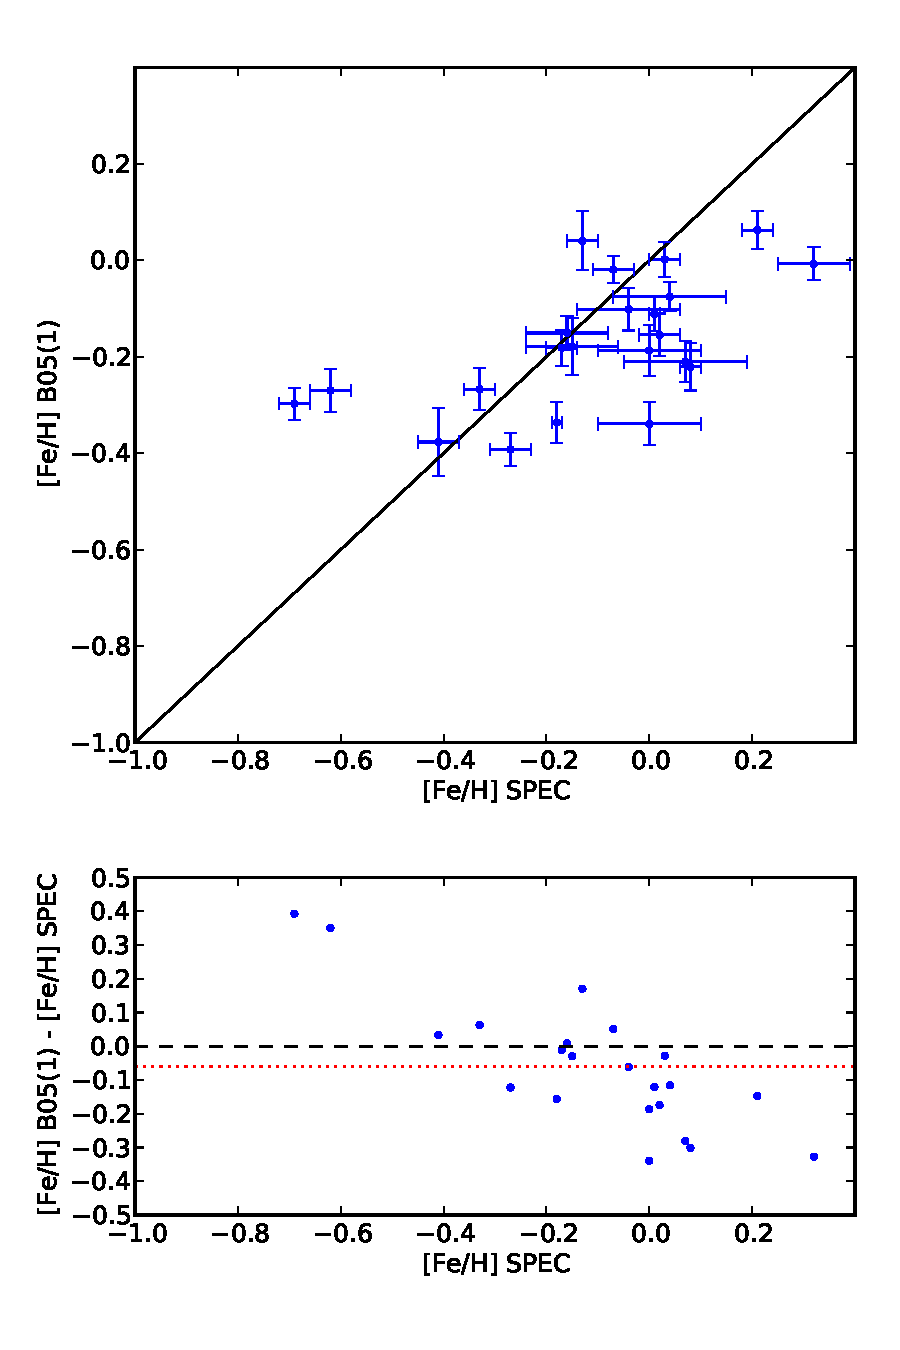
\includegraphics[scale=0.35]{pics/fehfehb051v3.pdf}}
%\subfigure[B05(2) Calibration]{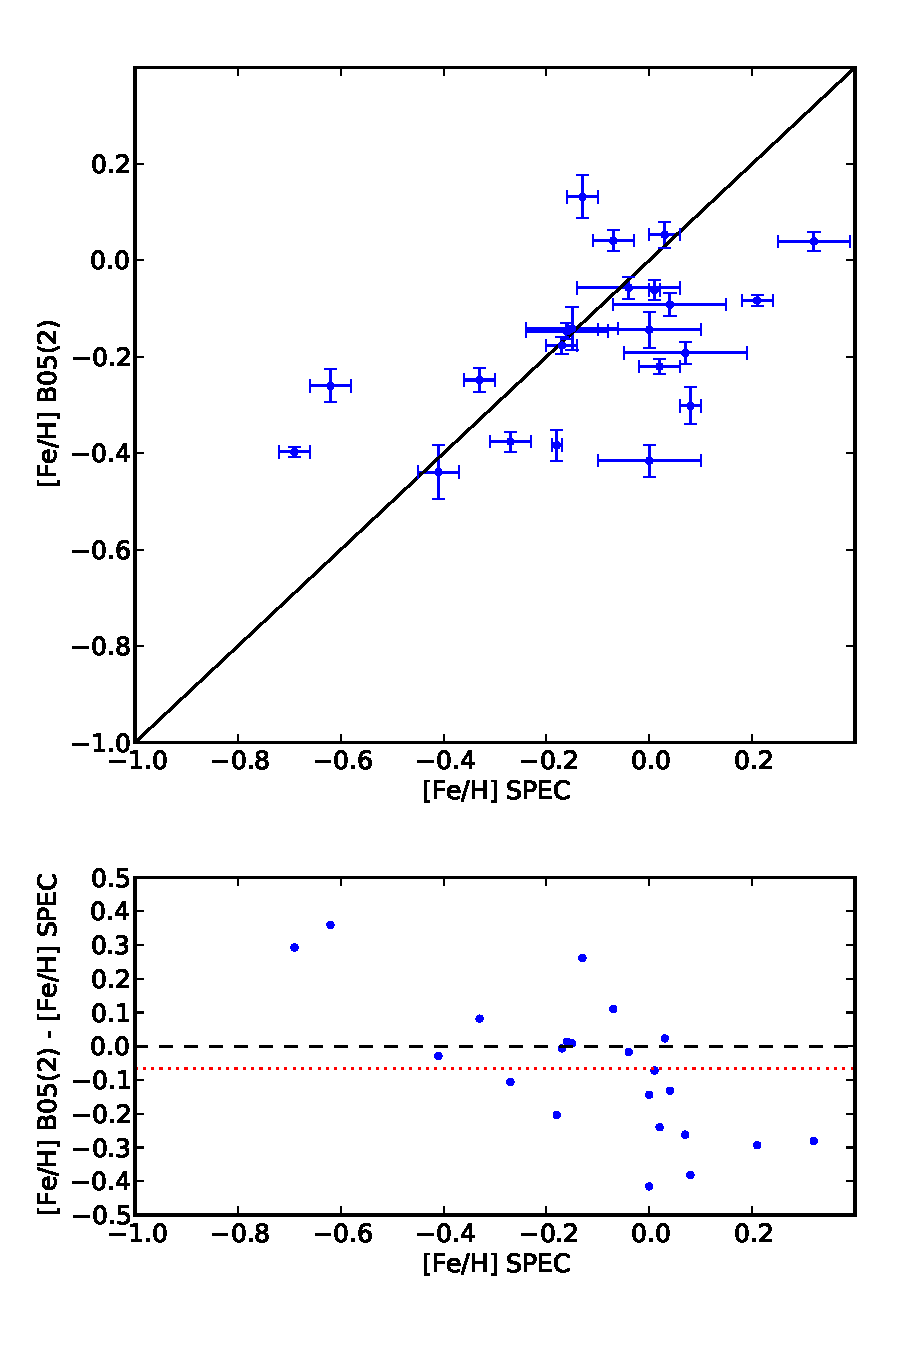
\includegraphics[scale=0.35]{pics/fehfehb052v3.pdf}}
%\subfigure[C08 Calibration]{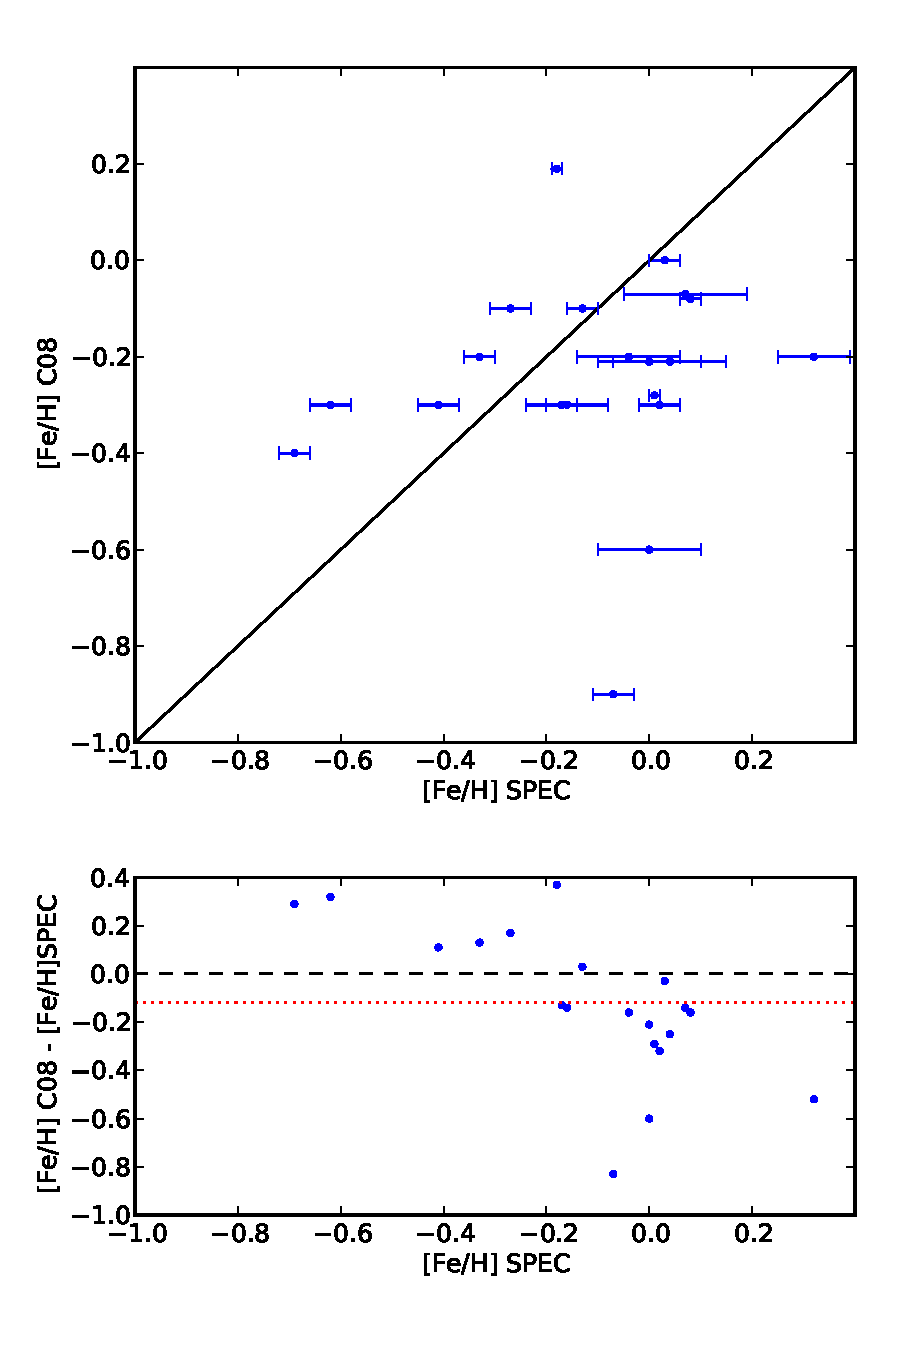
\includegraphics[scale=0.35]{pics/fehfehc08v3.pdf}}
%\subfigure[JA09 Calibration]{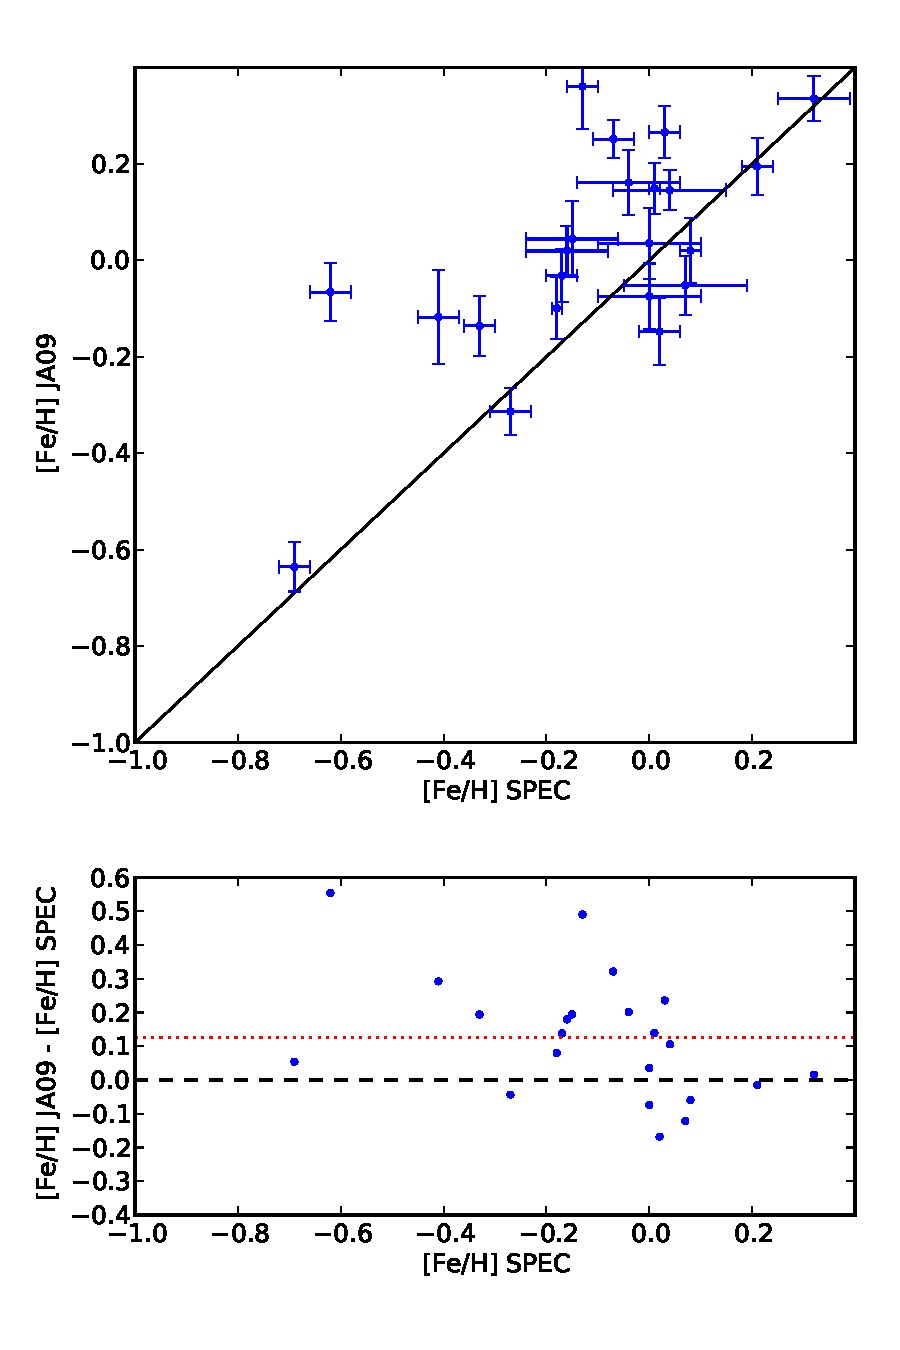
\includegraphics[scale=0.35]{pics/fehfehja09v3.pdf}}
%\subfigure[SL10 Calibration]{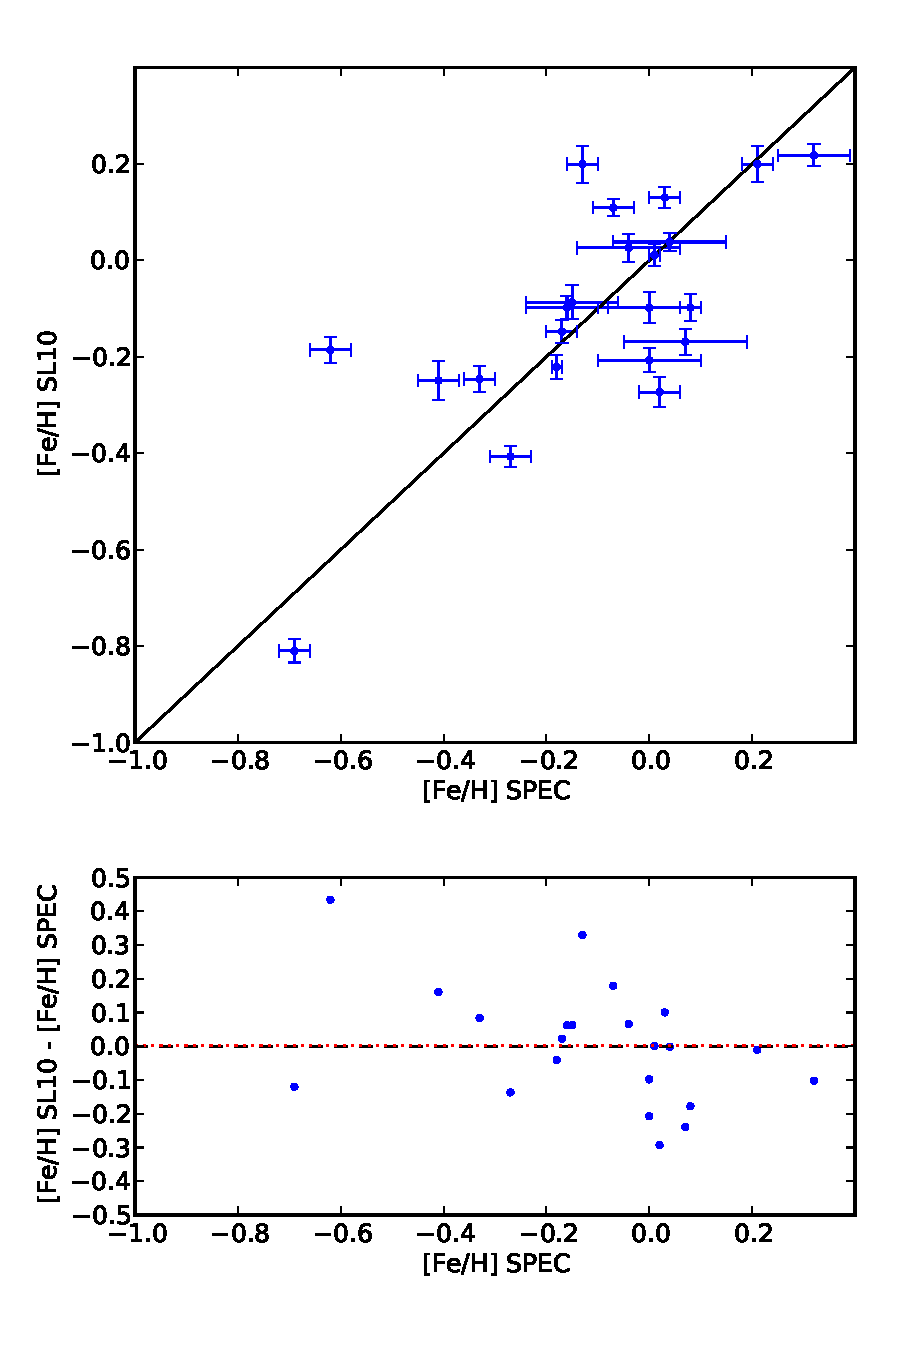
\includegraphics[scale=0.35]{pics/fehfehsl10v3.pdf}}
%\subfigure[SL10 Calibration (new fit) ]{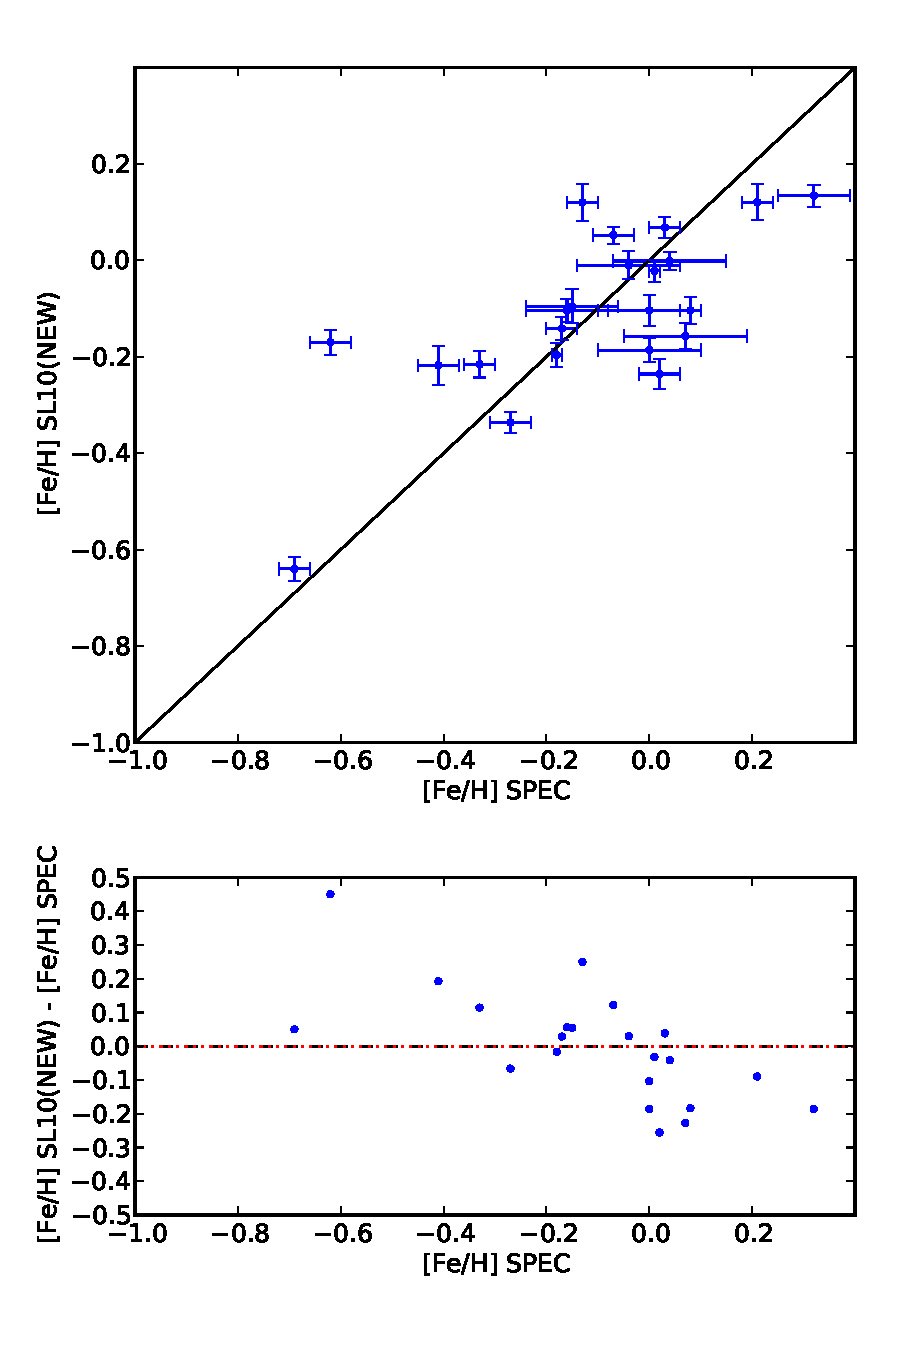
\includegraphics[scale=0.35]{pics/fehfehsl10newv3.pdf}}

%\end{center}
%\caption{[Fe/H] of the calibrations versus the spectroscopic metallicity. The tested calibrations are from \citet{Bonfils-2005} (a and b), \citet{Casagrande-2008} (c), \citet{Johnson-2009} (d), and \citet{Schlaufman-2010} (e). The (f) panel depicts the new fit of the calibration of \citet{Schlaufman-2010}. The blue dots with error bars represent the data points. The black line depicts a one to one relationship. The metallicity difference between the values of the calibrations and the spectroscopic measurements is shown below each [Fe/H]-[Fe/H] plot. The black dashed line is the zero point of the difference, and the red dotted line represents the average of the metallicity difference.  }
%\label{fehfeh}
%\end{figure*}

\begin{table*}[]
\caption{Metallicity values from spectroscopy and for the calibrations of \citet{Bonfils-2005}, \citet{Casagrande-2008}, \citet{Johnson-2009}, and \citet{Schlaufman-2010}. SL10(NEW) represents the [Fe/H] values of the new fit of \citet{Schlaufman-2010} calibration.}
\label{tablefehfeh}
\begin{center}
\begin{tabular}{r r r r r r r r r}

\hline
\hline

Primary & Secondary & \multicolumn{5}{c}{[Fe/H] [dex]}  \\
 & & Spectroscopic & B05(1) & B05(2) & C08 & JA09 & SL10 & SL10(NEW) \\
\hline
Gl53.1A & Gl53.1B & 0.07 & -0.21 & -0.19 & -0.07 & -0.05 & -0.17 & -0.16 \\
Gl56.3A & Gl56.3B & 0.00 & -0.34 & -0.42 & -0.21 & -0.07 & -0.21 & -0.19 \\
Gl81.1A & Gl81.1B & 0.08 & -0.22 & -0.30 & -0.08 & 0.02 & -0.10 & -0.10 \\
Gl100 & Gl100C & -0.27 & -0.39 & -0.38 & -0.10 & -0.31 & -0.41 & -0.34 \\
Gl105A & Gl105B & -0.17 & -0.18 & -0.18 & -0.30 & -0.03 & -0.15 & -0.14 \\
Gl140.1A & Gl140.1B & -0.41 & -0.38 & -0.44 & -0.30 & -0.12 & -0.25 & -0.22 \\
Gl157A & Gl157B & -0.13 & 0.04 & 0.13 & -0.10 & 0.36 & 0.20 & 0.12 \\
Gl173.1A & Gl173.1B & -0.33 & -0.27 & -0.25 & -0.20 & -0.14 & -0.25 & -0.22 \\
Gl211 & Gl212 & 0.04 & -0.08 & -0.09 & -0.21 & 0.15 & 0.04 & -0.00 \\
Gl231.1A & Gl231.1B & 0.01 & -0.11 & -0.06 & -0.28 & 0.15 & 0.01 & -0.02 \\
Gl250A & Gl250B & -0.15 & -0.18 & -0.14 & 99.00 & 0.04 & -0.09 & -0.10 \\
Gl297.2A & Gl297.2B & 0.03 & 0.00 & 0.05 & 0.00 & 0.27 & 0.13 & 0.07 \\
Gl324A & Gl324B & 0.32 & -0.01 & 0.04 & -0.20 & 0.34 & 0.22 & 0.13 \\
Gl559A & Gl551 & 0.21 & 0.06 & -0.08 & 99.00 & 0.19 & 0.20 & 0.12 \\
Gl611A & Gl611B & -0.69 & -0.30 & -0.40 & -0.40 & -0.64 & -0.81 & -0.64 \\
Gl653 & Gl654 & -0.62 & -0.27 & -0.26 & -0.30 & -0.07 & -0.19 & -0.17 \\
Gl783.2A & Gl783.2B & -0.16 & -0.15 & -0.15 & -0.30 & 0.02 & -0.10 & -0.10 \\
Gl797A & Gl797B & -0.07 & -0.02 & 0.04 & -0.90 & 0.25 & 0.11 & 0.05 \\
GJ3091A & GJ3092B & 0.02 & -0.15 & -0.22 & -0.30 & -0.15 & -0.27 & -0.24  \\
GJ3194A & GJ3195B & 0.00 & -0.19 & -0.14 & -0.60 & 0.04 & -0.10 & -0.10 \\
GJ3627A & GJ3628B & -0.04 & -0.10 & -0.06 & -0.20 & 0.16 & 0.03 & -0.01 \\
NLTT34353 & NLTT34357 & -0.18 & -0.34 & -0.38 & 0.19 & -0.10 & -0.22 & -0.20 \\


\hline
\end {tabular}
\end{center}
\end{table*}

Following the plots from Fig. \ref{fehfeh} and Table \ref{stats} we can observe that all calibrations fit the data reasonably, except in the case of C08 and JA09. These calibrations suffer from a big offset (-0.12 and 0.12 dex, respectively). The C08 calibration also has the worst rms, RMS$_{p}$ and R$^{2}_{ap}$ values. \textbf{The negative R$^{2}_{ap}$ value of the calibration of C08 means that this model is increasing the variance when compared to a constant model}. The B05(1) and the SL10 calibration have a similar value of RMS$_{p}$. However, regarding the offset, rms and the R$^{2}_{ap}$ values, the SL10 calibration has lower values (0.00 dex, 0.17 dex, and 0.30 respectively) than the ones from B05(1) calibration (-0.06 dex, 0.20 dex, and 0.33 respectively). This suggests that the best calibration for our sample is the one of SL10 and that this model is the best suited for explaining the variance of the data. 

Regarding our new fit of the SL10 calibration, we can observe that it is very similar to the original one, although a little bit tighter, with a slightly better rms. The R$^{2}_{ap}$ value can be considered equal (0.49 vs 0.50). We must note that, in the case of this new calibration, we used $p=2$ in Eq. (\ref{rmsp}).

The results of the bootstrap analysis, depicted in Table \ref{bootstrap}, show that the offset, rms, and RMS$_{p}$ values are robust, having small standard deviation values. However, the R$^{2}_{ap}$ standard deviation values imply a large variation of this parameter when using different sub-samples. This may mean that this parameter is not well suited for explaining the goodness-of-fit of a model, at least for small samples. %Nevertheless, the SL10 model has the highest R$^{2}_{ap}$ value (0.27) with the lowest dispersion (0.20). 
%The bootstrap analysis confirms that the SL10 is best calibration so far for predicting metallicities of M dwarfs.

The results also show that the B05(1) and JA09 models respectively underestimate and overestimate the metallicity in general, as it is clearly seen in Fig. \ref{fehfeh} in accordance with the findings of \citet{Schlaufman-2010}. 

\textbf{We must note the possible existence of a trend with spectroscopic [Fe/H], having a negative slope, for the B05(1), B05(2), C08, and SL10(NEW) calibrations. This may also be the case for the remaining calibrations, if we ignore the data point with the lowest value of [Fe/H]. We do not know the cause for this effect, but this may mean that the current models are missing a higher order trend. The B05(1), B05(2), and C08 calibrations also seem to overestimate the metallicity for spectroscopic [Fe/H] $< -0.4$. Regarding higher metallicities, above 0.2 dex, only the calibrations of JA09 and SL10 seem to accurately predict the spectroscopic metallicities: all the other calibrations underestimate the [Fe/H] value.}

%\textbf{We must note, however, that all calibrations seem to overestimate the metallicity for spectroscopic [Fe/H] $< -0.4$. Unfortunately, we only have one star in this region, but there is a hint that there may be a trend with a negative slope as a function of the spectroscopic metallicity in all the lower panels of Fig. \ref{fehfeh}. We do not know the cause for this trend. Regarding higher metallicities, above 0.2 dex, only the calibrations of JA09 and SL10 seem to accurately predict the spectroscopic metallicities: all the other calibrations underestimate the [Fe/H] value. }




%Regarding the remaining calibrations, the best one is the one from Sl10, which has a very small offset (-0.02 dex) and the smallest $rms$ value (0.19 dex) of all calibrations. The calibration of SL10 has the smallest value of $RMSp$ and $R^{2}_{ap}$. This means that this model is best suited for prediction as well as the best in explaining the variance of the data. This trends can be seen more clearly in Figs. \ref{residuals} and \ref{fehfeh}.



\textit{SL10 reports that the JA09 and the B05(1) calibrations have a R$^{2}_{ap}$ value of 0.06 and lower than 0.05, respectively. Our findings, however, show that the JA09 and B05(1) models can explain the variance of the data better than that, with a R$^{2}_{ap}$ value of 0.18 and 0.33 respectively. Therefore, the statement of SL10 that their model explains almost an order of magnitude more of the variance of the calibration sample, relative to the B05(1) model, is not confirmed. The discrepancy between the results may result from using different $p$  values in Eq. (\ref{rmsp}), as this may induce large changes in R$^{2}_{ap}$ . We used $p=0$ in Eq. (\ref{rmsp}) for all calibrations (except in the case of SL10(NEW)), whereas SL10 might have used other values.}

The calibration of \citet{Rojas-Ayala-2010} is reported as having a RMS$_{p}$ of only 0.02 and an R$^{2}_{ap} = 0.63$, with a dispersion of only 0.15 dex. Therefore, it would be very interesting to test it. Unfortunately, we were not able to do it because we lack the infrared spectra to measure the spectral indexes necessary for the calibration. We were able to do an external test, by comparing the measurements of the seven stars in common (Gl 212, Gl 231.1B, Gl 250B, Gl 324B, Gl611B, Gl783.2B, and Gl 797B). %with predicted [Fe/H] of 0.09, -0.05, -0.04, 0.3, and -0.09 dex respectively). 
We got a value of only 0.09 dex for the dispersion and a 0.04 dex offset between the spectroscopic measurements and \citet{Rojas-Ayala-2010} predicted metallicities. These numbers have little significance, but they may give a hint that the calibration is compatible with the spectroscopic measurements.



%%%METER AQUI UM PARAGRAFO SOBRE O SL10 E O NORDSTROM!

%%% O que dizer sobre a ROJAS?





\section {Discussion}
\label{discussion}

In this paper we tested the metallicity calibrations of \citet{Bonfils-2005}, \citet{Johnson-2009}, \citet{Casagrande-2008}, and \citet{Schlaufman-2010}, using precise metallicity determinations from binary/multiple systems and precise VRIJHK$_{S}$ photometry. We conclude that, at present, the best calibration is the one from \citet{Schlaufman-2010}: it has the lowest zero-point offset, dispersion, RMS$_{P}$ and has the highest R$^{2}_{ap}$. Unfortunately, we were not able to test the \citet{Rojas-Ayala-2010} calibration. Therefore, we cannot confirm or deny if this calibration is better than the one of \citet{Schlaufman-2010}. However, our limited external test with seven stars is encouraging and suggests that this calibration should be properly tested in the future.

We did a new fit of the SL10 expression and found that there are no significant differences between this new fit and the original SL10 calibration. The new fit is tighter but just by 0.01 dex (from 0.17 to 0.16 dex). We therefore conclude that the SL10 expression is valid for our sample. 

The impact of the precision of V photometry on the final precision of some of the calibrations (B05, JA09, SL10) have been recently discussed. In this paper we use precise V photometry, with an average precision of $\sim$ 0.02 mag, and conclude that the use of precise photometry does not impact the final dispersion of the mentioned calibrations: there is not a significant decrease of the obtained rms when compared to the dispersion reported in the original papers. 

The precise determination of metallicities of M dwarfs is very important in the understanding of the formation and evolution of planets around very low mass stars, as well as for studies about the star-planet connection. Some questions are left unanswered, such as which of the two parameters, [Fe/H] or mass, are the most important in the planet formation around M dwarfs, or whether the relation between the higher frequency of planets around stars that are richer in [Fe/H] is true for M stars or not. In order to answer these questions, a more precise metallicity determination is needed, either by doing a better calibration, or by exploring other approaches, such as using spectral indexes, like \citet{Woolf-2006}, and \citet{Rojas-Ayala-2010}, or by finding a way to directly measure the stellar parameters of M dwarfs, either empirically (e.g. \citeauthor{Woolf-2005} \citeyear{Woolf-2005}) or by using synthetic spectra (e.g. \citeauthor{Bean-2006} \citeyear{Bean-2006}). 

%In the near future, we aim to create a photometric metallicity calibration that can reach a precision of the order of $\sim$ 0.05 dex, as well as finding new ways to directly determine the metallicity and other parameters (such as effective temperature) from the M dwarf spectra. In this paper we did not address the planet-metallicity correlation, but we intend to do it in the future. 


%falar um pouco a dizer que infelizmente n podemos dizer grande coisa sobre os planetas mas que tentaremos responder a essas questoes num futuro proximo.
%FAZER bootstrap do sample e ESCREVER que a V photometry n e uma limitacao na determinacao do feh
%

\begin{acknowledgements}
%				      
%We thank the Swiss National Research Foundation (FNRS) and the Geneva 
%University for their continuous support to our planet search programmes. 
We would like to thank Luca Casagrande for kindly providing us the metallicities calculated from his calibration. We acknowledge the support by the European Research Council/European Community under the FP7 through Starting Grant agreement number 239953. NCS also acknowledges the support from Funda\c{c}\~ao para a Ci\^encia e a Tecnologia (FCT) through program Ci\^encia\,2007 funded by FCT/MCTES (Portugal) and POPH/FSE (EC), and in the form of grant reference PTDC/CTE-AST/098528/2008. VN would also like to acknowledge the support from FCT in the form of the fellowship SFRH/BD/60688/2009. 

\end{acknowledgements}


\bibliographystyle{aa}
\bibliography{mylib.bib}

\end{document}








%\begin{table}[b]
%\caption{Stellar parameters for \object{HD\,45652}.}
%\label{table:hd45652_star}
%\begin{tabular}{lcc}
%\hline\hline
%\noalign{\smallskip}
%Parameter  & Value & Reference \\
%\hline
%Spectral~type                   & K5/G8-K0              & Hipparcos/This Paper \\
%$m_v$                           & 8.1                   & Hipparcos \\
%$B-V$                           & 0.85                  & Hipparcos \\
%Distance~[pc]                   & 36$\pm$2              & Hipparcos \\
%$v~\sin{i}$~[km~s$^{-1}$]       & $<$2$\dagger$  	& This paper \\
%$\log{R'_\mathrm{HK}}$	        & $-$4.90$\pm$0.10$\dagger\dagger$      & This paper \\
%$T_{\rm eff}$~[K]               & 5312$~\pm~$68         & This paper \\
%$\log{g}$~[cgi]                 & 4.32$~\pm~$0.21       & This paper \\
%$\xi_{\mathrm{t}}$              & 0.89$~\pm~$0.09       & This paper \\
%${\rm [Fe/H]}$                  & $+$0.29$~\pm~$0.07    & This paper \\
%Mass~$[M_{\odot}]$              & 0.83$\pm$0.05         & This paper \\
%\hline
%\noalign{\smallskip}
%\end{tabular}
%\newline
%$\dagger$ From ELODIE spectra using a calibration similar to the one presented by \citet{Santos-2002a}\\
%$\dagger\dagger$ From SOPHIE spectra using a calibration similar to the one presented by \citet{Santos-2000a}
%\end{table}
%
%
%\begin{figure}[t]
%\resizebox{\hsize}{!}{\includegraphics{09402F2.eps}}
%\caption{{\it Top}: ELODIE (red circles), CORALIE (blue squares), and SOPHIE (magenta diamonds) 
%radial-velocities for HD\,45652 as a function of time, and the best Keplerian fit to the 
%data. {\it Bottom}: residuals of the fit.} 
%\label{fig:time}
%\end{figure}
%
%
